\section{Auswertung}

\tabref{tab:elemente_kalph_kbeta} zeigt noch einmal zusammengefasst die durch die Analysesoftware ermittelten Energiewerte der $K_{\alpha}$- und $K_{\beta}$-Linien der untersuchten Elemente. Die Linien sind auch in \abbref{fig:elemente_metalle} in den jeweils zugeordneten Elementsymbolen beziehungsweise Farben zu finden. Zur Kalibrierung der Energieskala assoziierten wir die Energie der $K_\alpha$-Linie von Eisen von $6.40\si{\kilo\electronvolt}$ mit dem Kanal $111 \pm 3$ und die Energie $17.48\si{\kilo\electronvolt}$ der $K_\alpha$-Linie von Molybdän mit dem Kanal $279 \pm 3$.


\begin{table}[H]
  \centering
  \begin{tabular}{|c|c|c|c c|c c|}
      \hline
      \multirow{2}{*}{\#} & \multirow{2}{*}{Element}  & \multirow{2}{*}{Farbe}  & \multicolumn{2}{c|}{$K_{\alpha}$ $[\si{\kilo\electronvolt}]$}  & \multicolumn{2}{c|}{$K_{\beta}$ $[\si{\kilo\electronvolt}]$} \\\cline{4-7}
      && & $E_{\alpha}$ & $\Delta E_{\alpha}$ & $E_{\beta}$ & $\Delta E_{\beta}$ \\
      \hline
      1  & Molybdän  & schwarz    & 17.46 & 0.18 & 19.57 & 0.17 \\
      2  & Eisen     & rot        & 6.38  & 0.17 & 7.03  & 0.42 \\
      3  & Nickel    & blau       & 7.46  & 0.18 & 8.26  & 0.21 \\
      4  & Zink      & lila       & 8.64  & 0.18 & 9.59  & 0.16 \\
      5  & Zirconium & cyan       & 15.78 & 0.18 & 17.67 & 0.19 \\
      6  & Titan     & ultramarin & 4.44  & 0.19 & 4.44  & 0.19 \\
      7  & Kupfer    & pink       & 8.04  & 0.17 & 8.91  & 0.14 \\
      8  & Silber    & rostbraun  & 21.89 & 0.21 & 24.59 & 0.18 \\
      \hline
  \end{tabular}
  \caption{Energien der $K_{\alpha}$- und $K_{\beta}$-Linien der untersuchten Elemente.}
  \label{tab:elemente_kalph_kbeta}
\end{table}

\begin{figure}[H]
  \centering
  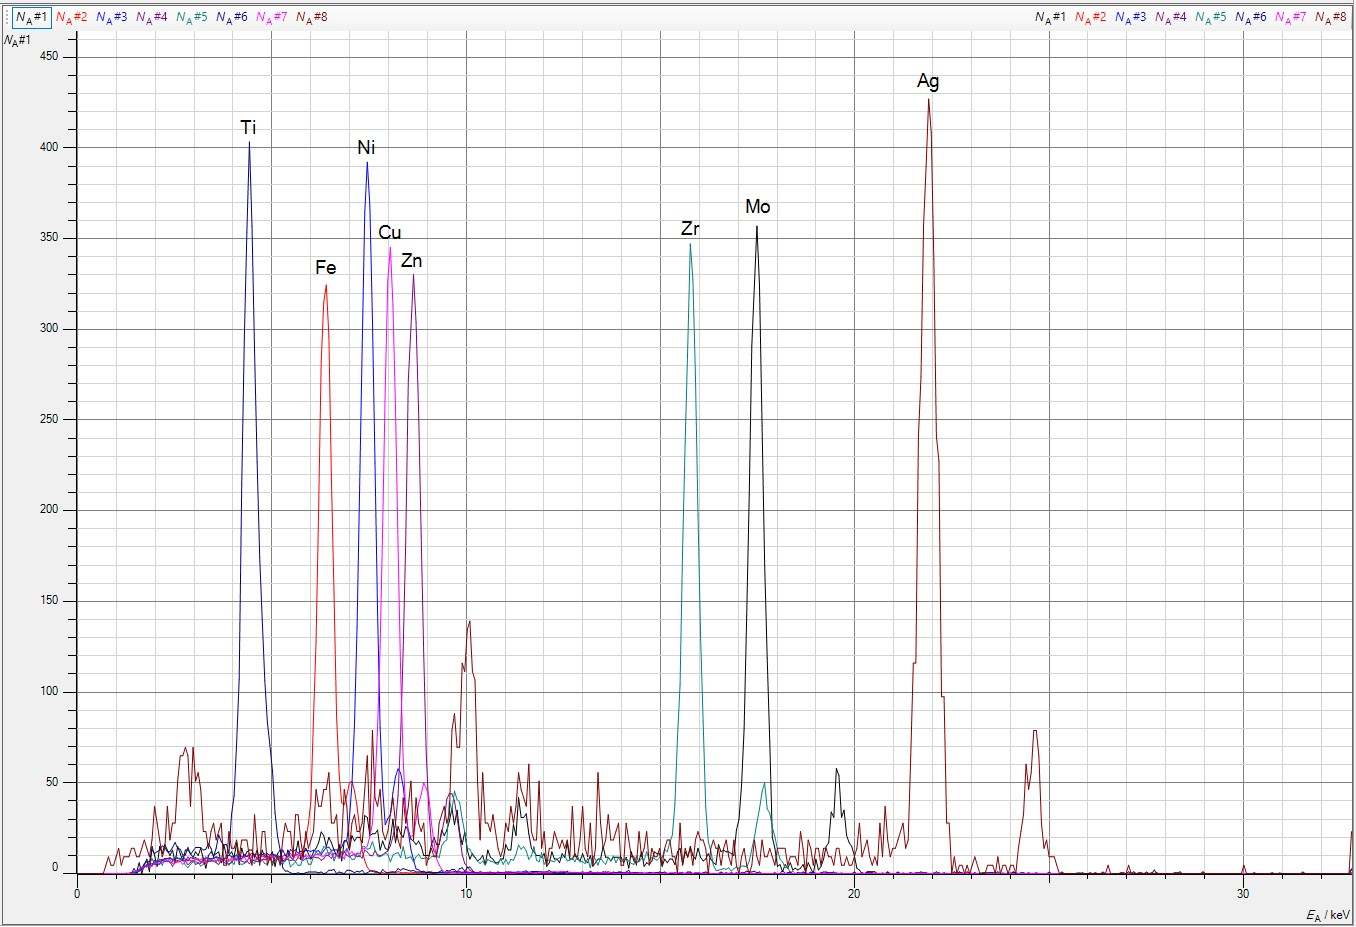
\includegraphics[width=\textwidth]{files/elemente_metalle.jpg}
  \caption{Röntgenfluoreszenzspektren der untersuchten Elemente. Zu sehen sind die Häufigkeiten, zu welcher die Energien gemessen wurden.}
  \label{fig:elemente_metalle}
\end{figure}
\newpage\noindent
Wir möchten nun die gemessenen Energiewerte je für die $K_{\alpha}$- und die $K_{\beta}$-Linien der Elemente als Funktion der Kernladungszahl betrachten und an diese die Funktion
\begin{align}
  \sqrt{E_{\alpha(\beta)}} = \sqrt{E_R} (Z - \sigma_{n_1, n_2}) \sqrt{\qty(\frac{1}{n_1^2} - \frac{1}{n_2^2})} = f(Z; \sqrt{E_R}, \sigma_{n_1, n_2})\label{eq:sqrt_energy_fit_function}
\end{align}
mit den Parametern $\sqrt{E_R}$ und $\sigma_{n_1, n_2}$ anpassen. Hierzu berechnen wir zunächst die Wurzeln der Energiewerte aus \tabref{tab:elemente_kalph_kbeta} nach der Formel
\begin{align}
  \sqrt{E_{\alpha(\beta)}} \pm \Delta \sqrt{E_{\alpha(\beta)}} = \sqrt{E_{\alpha(\beta)}} \pm \frac{1}{\sqrt{E_{\alpha(\beta)}}} \Delta E_{\alpha(\beta)}.
\end{align}

Wir betrachten zunächst die $K_{\alpha}$-Linie. Diese entspricht dem Übergang $2 \to 1$, somit gilt $n_2 = 2$, $n_1 = 1$ und wir suchen $\sigma_{12}$, sowie $\sqrt{E_R}$. \abbref{fig:K_alpha_vs_Z_with_fit} zeigt die Wurzeln ermittelten Energiewerte mit Fehlern aufgetragen über der Kernladungszahl der Elemente, sowie die optimierte Funktion \eqref{eq:sqrt_energy_fit_function} mit den entsprechenden genannten Parametern.

\begin{figure}[H]
  \centering
  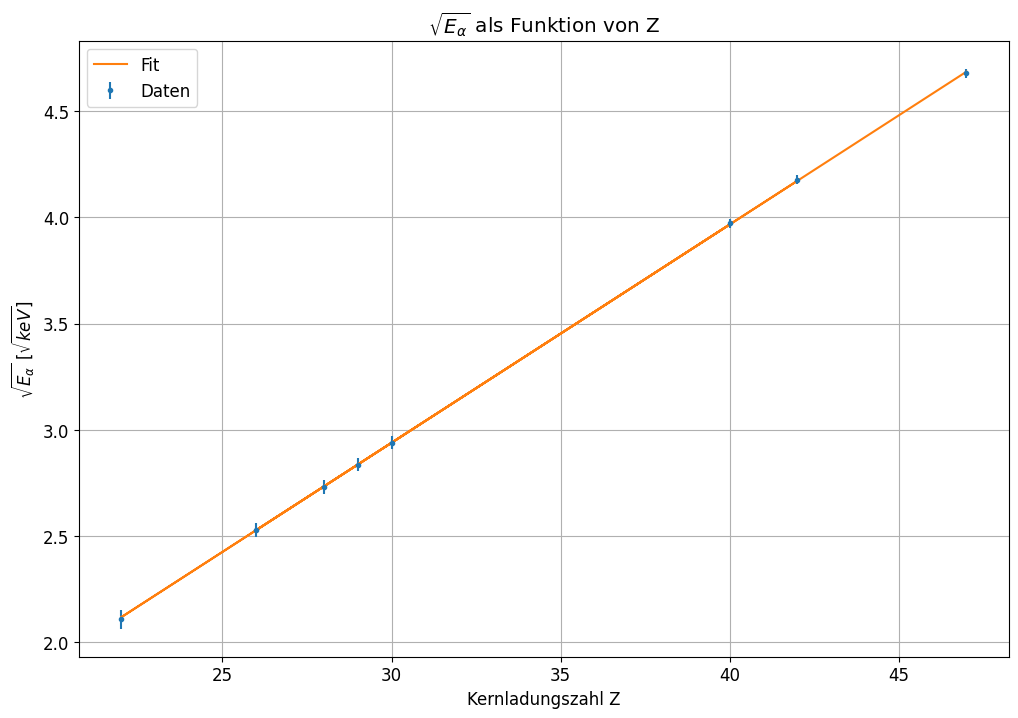
\includegraphics[width=\textwidth]{files/K_alpha_vs_Z_with_fit.png}
  \caption{$\sqrt{E_{\alpha}}$ als Funktion der Kernladungszahl $Z$ der untersuchten Elemente mit Fit der Funktion \eqref{eq:sqrt_energy_fit_function}.}
  \label{fig:K_alpha_vs_Z_with_fit}
\end{figure}

Die optimierten Werte der Parameter lauten
\begin{align}
  \sqrt{E_R} &= (0.1188 \pm 0.0015) \si{\kilo\electronvolt},\\[1em]
  \sigma_{12} &= 1.4 \pm 0.5.
\end{align}

Wir quadrieren $\sqrt{E_R}$ und bestimmen so einen ersten Wert für die Rydberg-Energie von
\begin{align}
  E_R &= (14.1 \pm 0.4) \si{\electronvolt}.
\end{align}

Die gleiche Prozedur führen wir nun noch einmal für die Energien der $K_{\beta}$-Linien durch. Hierbei betrachten wir Übergang $3\to1$, es gilt also $n_2 = 3$, $n_1 = 1$ und wir suchen $\sigma_{13}$, sowie erneut $\sqrt{E_R}$. \abbref{fig:K_beta_vs_Z_with_fit} zeigt erneut die Wurzeln ermittelten Energiewerte mit Fehlern über der Kernladungszahl, sowie die optimierte Funktion \eqref{eq:sqrt_energy_fit_function} mit den entsprechenden Parametern.


\begin{figure}[H]
  \centering
  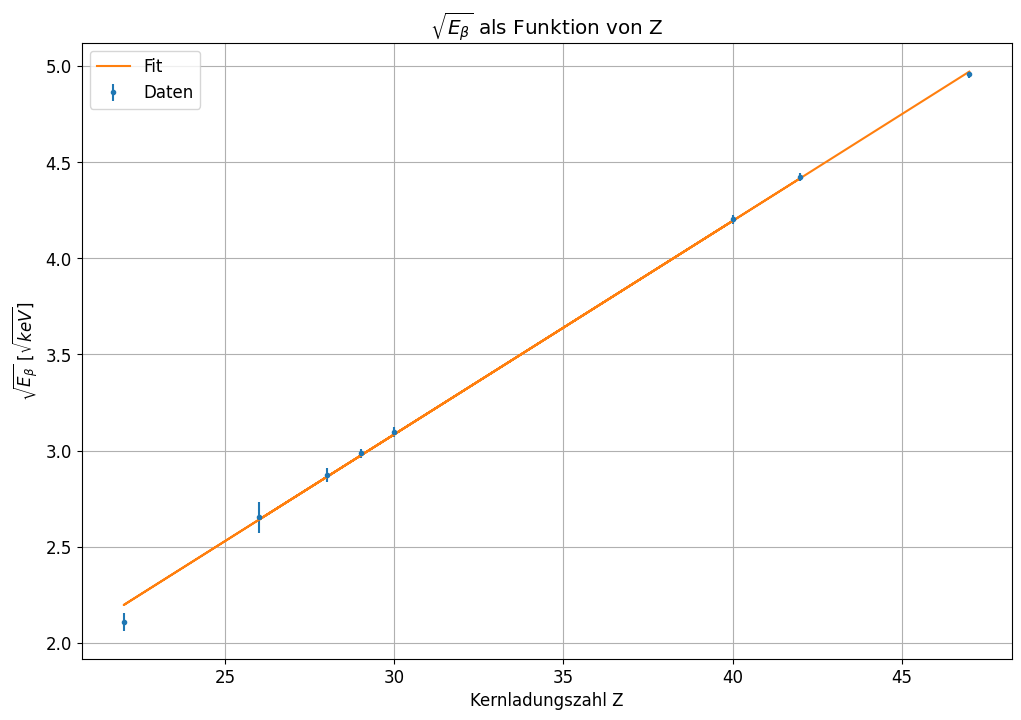
\includegraphics[width=\textwidth]{files/K_beta_vs_Z_with_fit.png}
  \caption{$\sqrt{E_{\beta}}$ als Funktion der Kernladungszahl $Z$ der untersuchten Elemente mit Fit der Funktion \eqref{eq:sqrt_energy_fit_function}.}
  \label{fig:K_beta_vs_Z_with_fit}
\end{figure}

Aus dem Fit erhalten wir hierbei die optimierten Parameter
\begin{align}
  \sqrt{E_R} &= (0.1178 \pm 0.0013) \si{\kilo\electronvolt},\\[1em]
  \sigma_{13} &= 2.2 \pm 0.4.
\end{align}

Wir quadrieren erneut $\sqrt{E_R}$ und erhalten so einen weiteren Wert für die Rydberg-Energie von
\begin{align}
  E_R &= (13.87 \pm 0.21) \si{\electronvolt}.
\end{align}
\newpage\noindent
Für den zweiten Versuchsteil haben wir die Röntgenfluoreszenzspektren verschiedener Metalllegierungen aufgezeichnet. Anhand der in den Spektren sichtbaren $K_{\alpha}$- und $K_{\beta}$-Peaks haben wir diesen die entsprechenden reinen Metalle zugeordnet, welcher in der Legierung enthalten sind. Die Spektren sind in den folgenden Abbildungen (\ref{fig:legierung1}) bis (\ref{fig:legierung5}) zu sehen.
\vspace*{5em}

\begin{figure}[H]
  \centering
  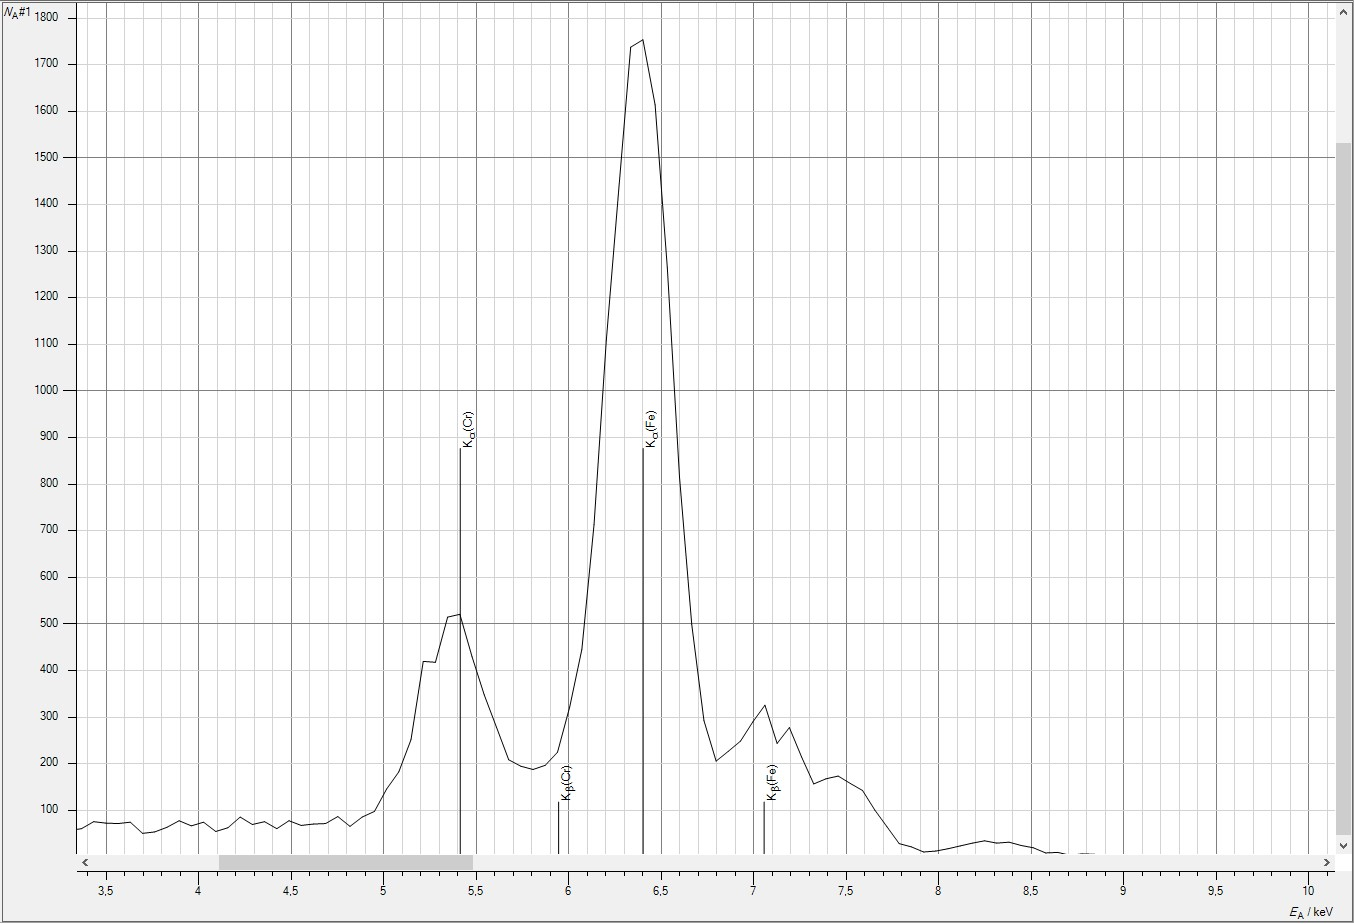
\includegraphics[width=\textwidth]{files/legierung1.jpg}
  \caption{Probe 1, Legierung: Eisen, Chrom = Ferrochrom(?)}
  \label{fig:legierung1}
\end{figure}


\begin{figure}[H]
  \centering
  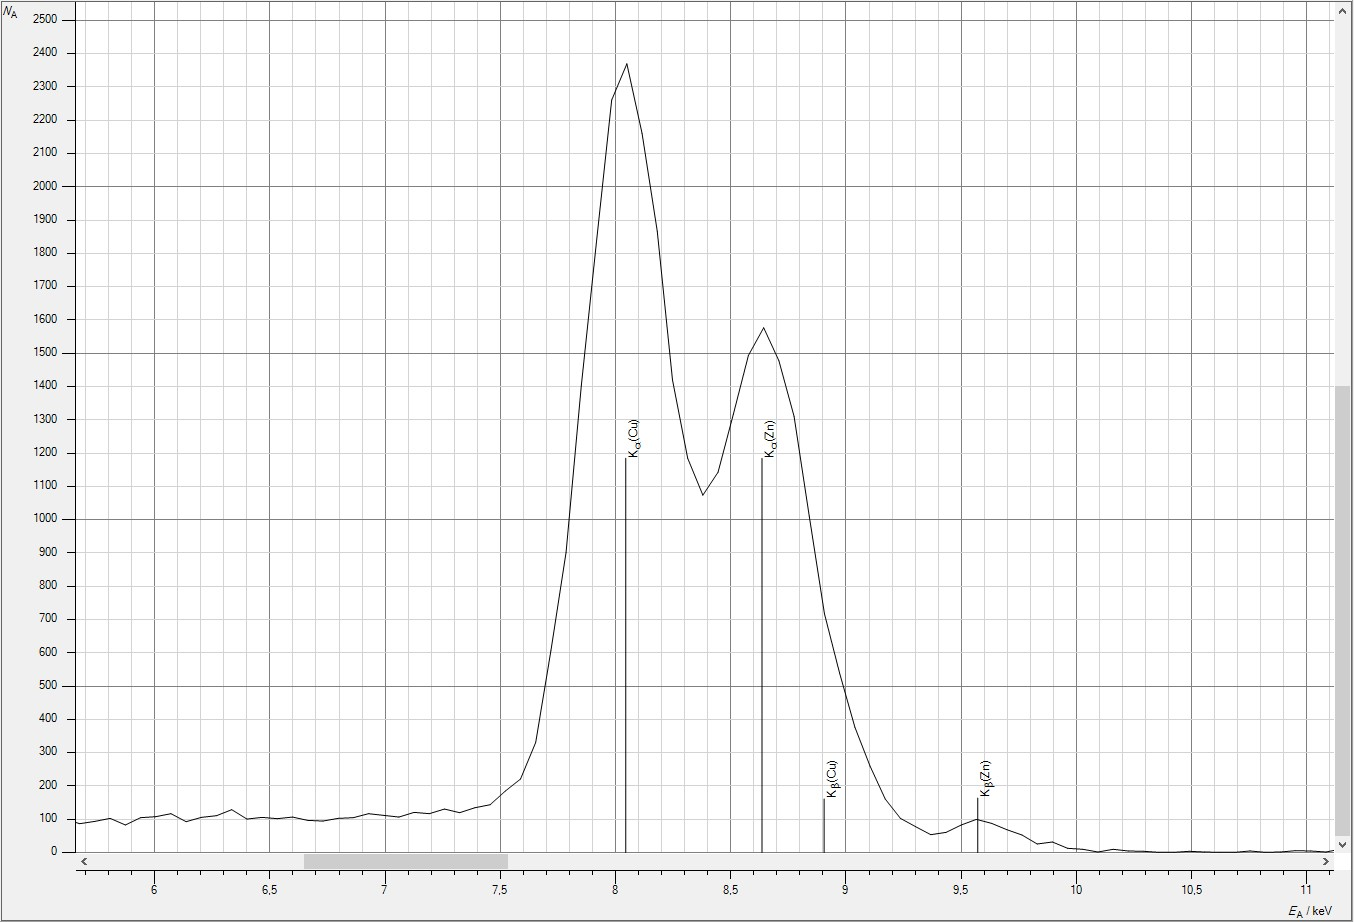
\includegraphics[width=\textwidth]{files/legierung2.jpg}
  \caption{Probe 2, Legierung: Kupfer, Zink = Messing}
  \label{fig:legierung2}
\end{figure}

\begin{figure}[H]
  \centering
  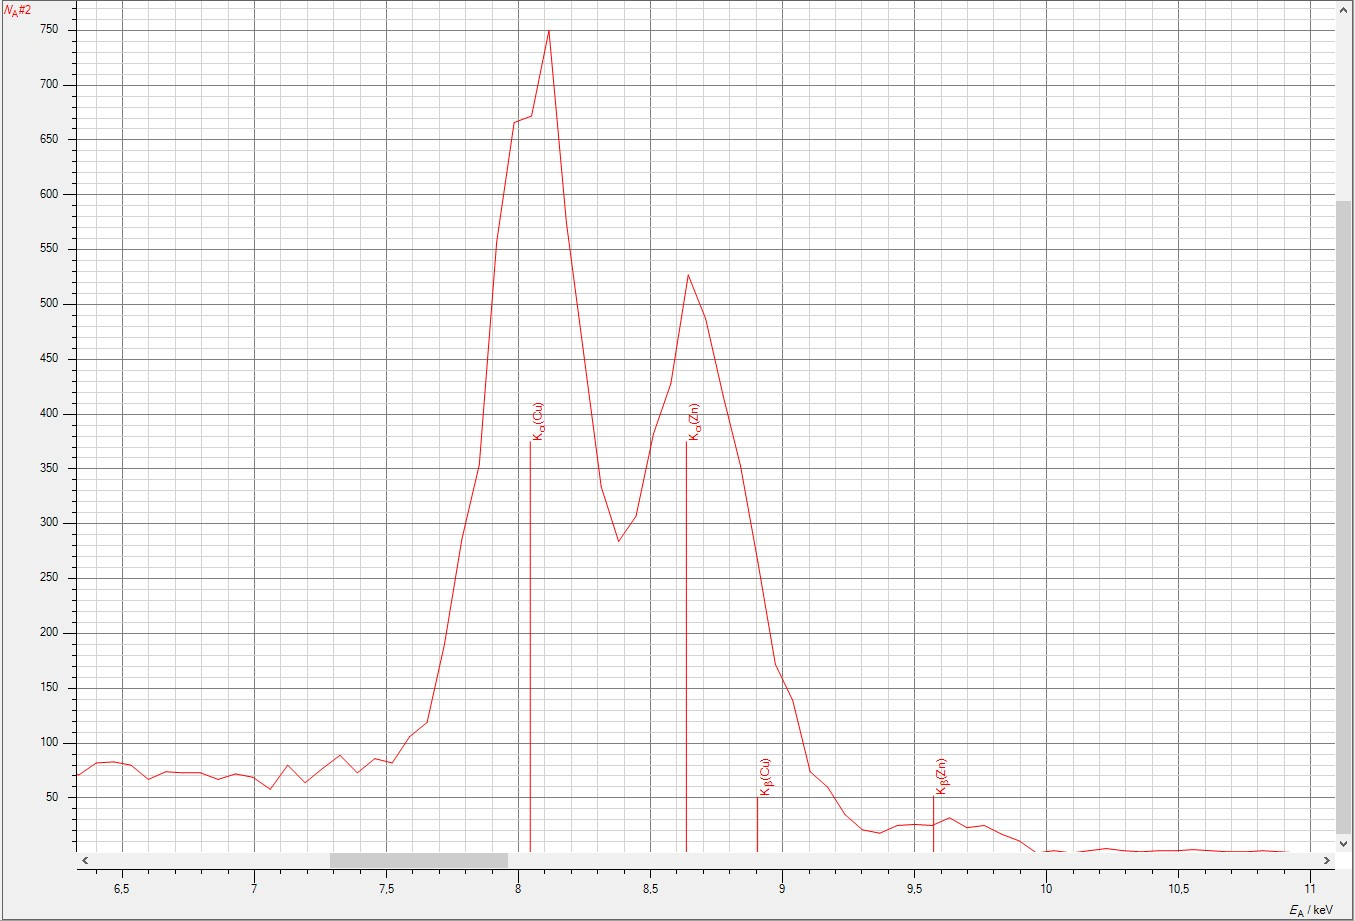
\includegraphics[width=\textwidth]{files/legierung3.jpg}
  \caption{Probe 3, Legierung: Kupfer, Zink = Messing}
  \label{fig:legierung3}
\end{figure}

\begin{figure}[H]
  \centering
  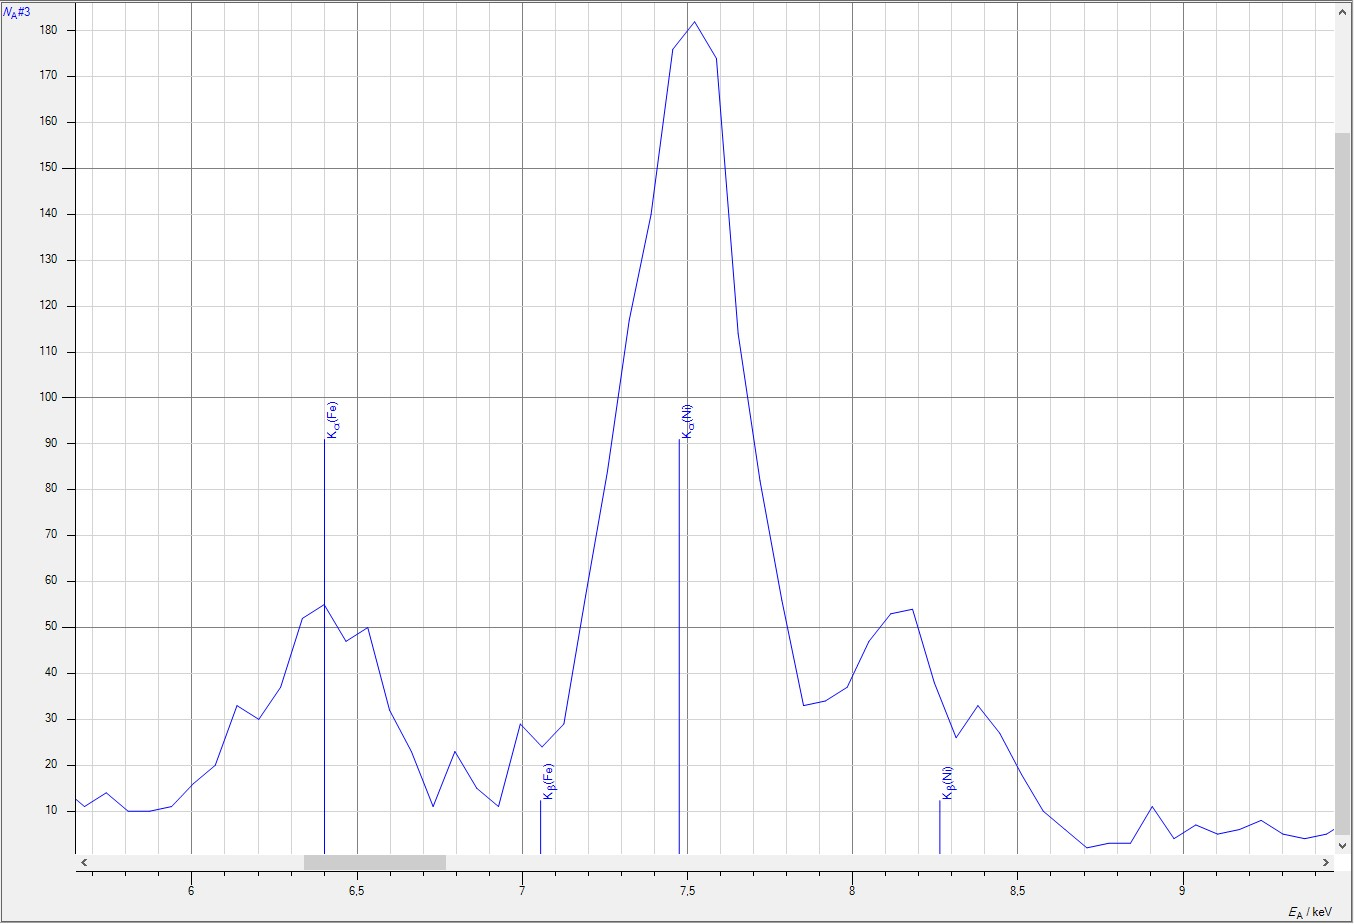
\includegraphics[width=\textwidth]{files/legierung4.jpg}
  \caption{Probe 4, Legierung: Eisen, Nickel = Invar(?)}
  \label{fig:legierung4}
\end{figure}


\begin{figure}[H]
  \centering
  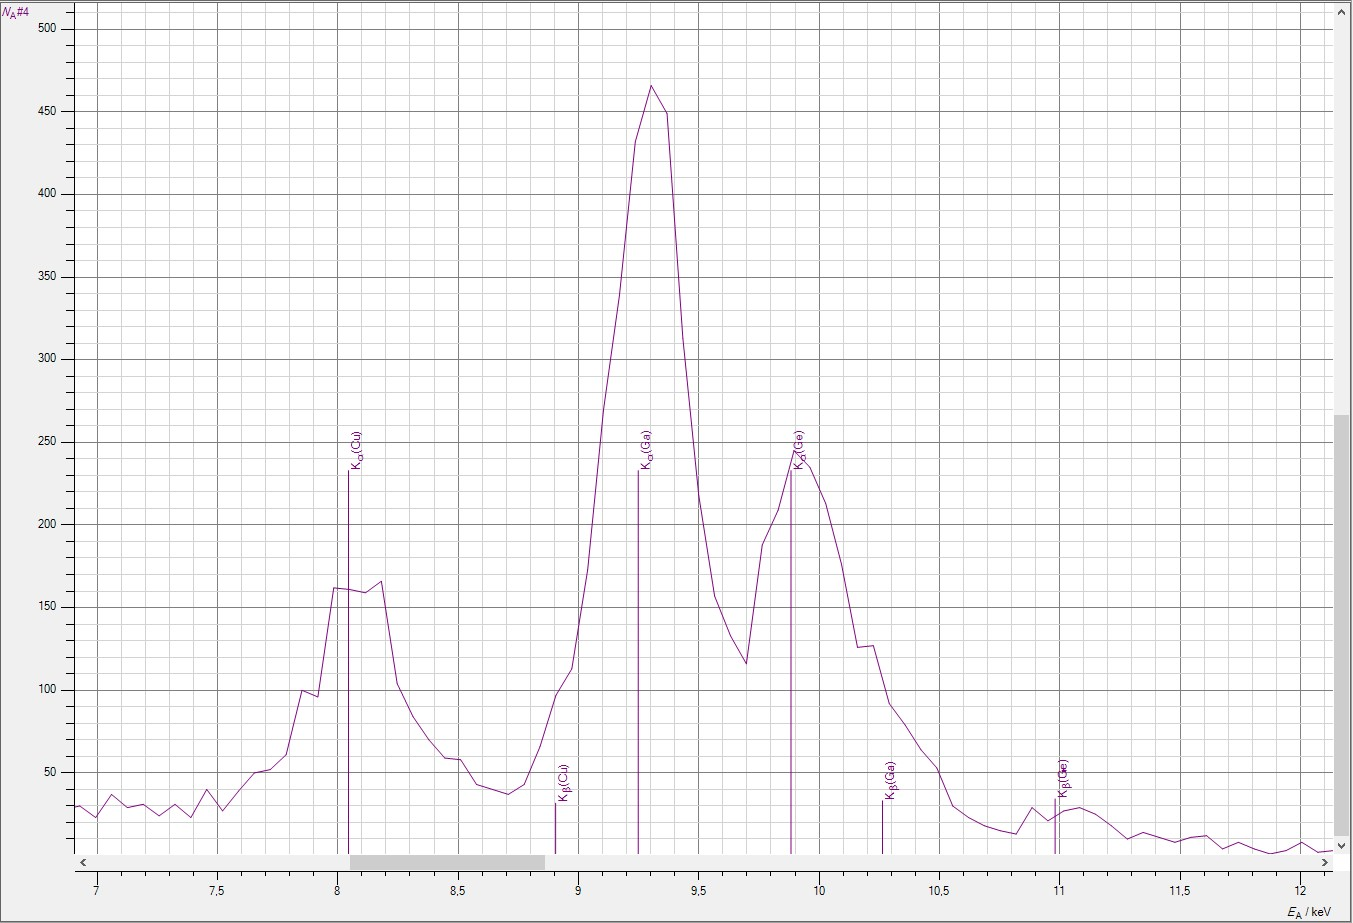
\includegraphics[width=\textwidth]{files/legierung5.jpg}
  \caption{Probe 5, Legierung: Kupfer, Gallium, Germanium}
  \label{fig:legierung5}
\end{figure}
